\documentclass[12pt,a4paper]{article}
\usepackage[utf8]{inputenc}%agregado
\usepackage{amsmath}
\usepackage{graphicx}
\usepackage{amssymb}%agregado
\usepackage{amsthm}%agregado
\usepackage{color}	

%---
\usepackage[breaklinks=true,backref=page]{hyperref}

\usepackage[english]{babel}%agregado
%\usepackage{natbib}%agregado para ref apa
\usepackage[square,numbers]{natbib}%agregado ref apa

%\usepackage[section,nottoc]{tocbibind}%poner referenica en la tabla de contenidos
\usepackage[nottoc]{tocbibind}%poner referenica en la tabla de contenidos


\usepackage{multirow}%para unir filas


\usepackage{amsthm}
%\theoremstyle{plain}
%\newtheorem{thm}{Teorema}[section]
%\newtheorem{lem}[thm]{Lema}
%\newtheorem{prop}[thm]{Proposición}
%\newtheorem{cor}[thm]{Corolario}
\theoremstyle{plain}% default
\newtheorem{thm}{Theorem}[section]
\newtheorem{lem}[thm]{Lemma}
\newtheorem{prop}[thm]{Proposition}
\newtheorem*{cor}{Corollary}
%\newtheorem*{KL}{Klein’s Lemma}

\theoremstyle{definition}
\newtheorem{defn}{Definición}[section]
%\newtheorem{conj}{Conjectura}[section]
\newtheorem{exmp}{Ejemplo}[section]
\newtheorem{xca}[exmp]{Ejercicio}

\theoremstyle{remark}
\newtheorem*{rem}{Observación}
\newtheorem*{note}{Note}
\newtheorem{case}{Case}


\newcommand{\minitab}[2][l]{\begin{tabular}{#1}#2\end{tabular}}%para la tabla




%\title{Distribución de parásitos por sexo y la probabilidad de apareamiento}
\title{Basic modelling macroparasitic diseases}
\author{Gonzalo Maximiliano LOPEZ$^{1,3}$, Juan Pablo APARICIO$^{1,2,4}$\\
	\\
	{\small $^1$ Instituto de Investigaciones en Energ\'ia no Convencional (INENCO),} \\ {\small Consejo Nacional de Investigaciones Cient\'ificas y T\'ecnicas (CONICET),}\\
	{\small Universidad Nacional de Salta, Av. Bolivia 5150, 4400 Salta, Argentina.}\\
	$^2${\small Simon A. Levin Mathematical, Computational and Modeling Sciences Center,} \\ {\small Arizona State University, PO Box 871904 Tempe, AZ 85287-1904, USA}\\
	{\small $^3$ Departamento de Matem\'atica, Universidad Nacional de Salta (UNSa),}\\{\small Facultad de Ciencias Exactas, Av. Bolivia 5150, 4400 Salta, Argentina.}\\
	{\small $^4$ Corresponding author: juan.p.aparicio@gmail.com}}
\date{}

%\\
%{\small Corresponding author: juan.p.aparicio@gmail.com}}





 
%---para escribir las letras griegas en negrita
\usepackage{bm}

\usepackage{subfig}%para el subfloat

\usepackage{float}
\floatstyle{plaintop}
\restylefloat{table}





%---
%-----Comandos-----
\newcommand{\nc}{\newcommand}
\nc{\R}{\mathbb{R}}
\nc{\N}{\mathbb{N}}
\nc{\pa}{\partial}
\nc{\F}{\mathfrak{H}}
\nc{\f}{\mathfrak{f}}

%\l

\newcommand{\vect}[1]{\bm{#1}}%\usepackage{bm}

\begin{document}
\maketitle
\begin{abstract}
	\addcontentsline{toc}{section}{Abstract}
	
	COMPLETAR
	
	Keywords: Macroparasite; Mathematical models; Negative binomial distribution; Zero-inflated Model.
\end{abstract}
\tableofcontents
\tableofcontents
\section{Introduction}
	%{\color{red}PROFE: en este primer párrafo no entendí lo que me corrigió}
%	Las geohelmintiasis 
%	%o comúnmente conocidas como lombrices intestinales y 
%	son las infecciones más comunes a nivel mundial.
%	Se estima que 5300 millones de personas en todo el mundo, incluidos mil millones de niños en edad escolar, viven en áreas donde estas infecciones son endémicas \cite{pullan2012global}.
% 	Los agentes causales de estas infecciones son los parásitos nematodos intestinales Ascaris \textit{lumbricoides}, Trichuris \textit{trichiura} y las uncinarias (Necator americanus y Ancylostoma duodenale).
% 	
% 	Las infecciones por geohelmintos se tratan con fármacos de administración oral siendo los más comunes Albendazol y Mebendazol,
% 	%medicamentos antihelmínticos
% 	que se distribuyen a las poblaciones afectadas en campañas o programas de desparasitación masiva. 
% 	%La OMS recomienda tratamientos masivos para todos los grupos de riesgo en las comunidades donde la infección es endémica, especialmente
% 	%las mujeres en edad fértil, los niños en edad preescolar y los niños en edad escolar \cite{who2006preventive}.
% 	Comúnmente estas campañas están dirigidas a las poblaciones más afectadas,  
% 	las mujeres en edad fértil, los niños en edad preescolar y los niños en edad escolar \cite{who2006preventive}.
% 	%niños de 2 a 14 años de edad \cite{pizzi2007geohelmintiosis}. 
% 	%Además 
 	
 	Mathematical models play an important role in understanding the transmission and impact of macroparasite infection control measures \cite{anderson1992infectious,anderson2014coverage,truscott2016soil}.
	% 	The first work on the theory of helminth infection was published in the 1960s by Tallis and Leyton by developing stochastic models of transmission targeting nematode parasites of sheep and cattle \cite{tallis1966stochastic,leyton1968stochastic, tallis1969stochastic}.
	The first works on the theory of helminth infection was published in the 1960s by Tallis and Leyton by developing stochastic models of nematode parasite transmission in sheep and cattle \cite{leyton1968stochastic,tallis1966stochastic,tallis1969stochastic}.
 	
 	%Simultaneously Macdonald identified that a consequence of sexual reproduction of distributed parasites within individual hosts was the inability to generate fertile infectious material when prevalence is low \cite{macdonald1965dynamics}.
 	
 	Simultaneously Macdonald show that a consequence of sexual reproduction of distributed parasites within individual hosts was the inability to generate fertile infectious material when prevalence is low \cite{macdonald1965dynamics}.
 	
 	%This phenomenon introduces the idea of ​​two stable states, endemic infection and extinction separated by a breakpoint; that is, a level of intensity or prevalence of infection below which the parasites generate insufficient fertile infectious material to maintain a viable transmission cycle.
 	
% 	Anderson and May then introduced much more general descriptions of helminth population dynamics. They developed descriptions for a model based on host age, distribution of parasite numbers per host, density dependence of egg production, and sexual mating functions that depend on parasite distribution and feeding habits. mating \cite{anderson1982population,anderson1992infectious}.
 	
 	Anderson and May then introduced much more general descriptions of helminth population dynamics. They developed descriptions for a model based on host age, distribution of parasite numbers per host, density dependence of egg production, and sexual mating functions that depend on parasite distribution and reproductive habits \cite{anderson1982population,anderson1992infectious}.
 	
 	In this article we develop an analytical framework to describe the transmission dynamics of parasitic infections. We first analyzed the epidemiological patterns of these infections. We studied the individual distribution of the parasites in the community of hosts and also the distribution by sex of the parasites. From this we obtain expressions for the fertilized egg production and the mating probability of parasites. For these last variables we consider a density-dependent fecundity, a characteristic of helminth parasites. 
 	
 	Then we present the calculations of the equilibrium values of the model and 
 	the basic reproduction number $R_0$ defined for case of macroparasitos as the average number of new parasite offsprings caused by one typical parasite, from one generation to the next. 
 	%We show that our model has a saddle-node bifurcation.
 	We show that our model has a saddle node bifurcation.
 	Finally we show all the analytical results supported by numerical analysis.
 	
% 	Esta infecciones están ampliamente distribuidas en áreas tropicales y subtropicales, están ligadas a la falta de saneamiento y ocurren en poblaciones pobres. En la Región de América Latina se estima que hay cerca de 46 millones de niños en edad pre-escolar y escolar en riesgo de sufrir infecciones por geohelmintos. Los estudios indican que alrededor 30\% de la población está infectada \cite{PAHO/WHO2003}. 
 	
% 	En Argentina se registraron prevalencias variando entre cero hasta cercanas a 90\% \cite{saboya2011prevalence}, lo que refleja la heterogeneidad de su distribución en nuestro país. Una revisión sistemática de los estudios poblacionales publicados entre 1980 y 2011 \cite{socias2014geohelmintiasis}, muestra que la prevalencia para Ascaris lumbricoides 0-67\%, Uncinarias 0-90\%, Trichuris trichiura 0-24.5\%, Strongyloides stercoralis 0-83\%.
% 	Históricamente, las geohelmintiasis se han considerado endémicas en las
% 	zonas del norte del país, donde se encuentran las condiciones climáticas y socio
% 	ambientales que favorecen la perpetuación de estas infecciones. Sin embargo, también se
% 	muestran focos de alta prevalencia en el centro del país, como en Santa Fe \cite{lura2002prevalence} ($>$ 37\%), Provincia de Buenos Aires, en población de asentamientos periurbanos de
% 	la ciudad de La Plata \cite{gamboa2009associations} (25\% al 35\%), y en la ciudad de Brandsen del 19.2\% \cite{zonta2007parasitosis}.
 	
% 	El impacto de estas infecciones en el hospedador rara vez es agudo y suele ser a largo plazo y de naturaleza acumulativa. Las infecciones por geohelmintos rara vez causan la muerte, pero las infecciones crónicas e intensas pueden contribuir a la desnutrición, la anemia y también pueden afectar negativamente el desarrollo físico y cognitivo en la infancia \cite{brooker2010global}.%(Brooker et al., 2010; Banco Mundial, 2003; Albonico et al., 2008). 
	
%	La política de la Organización Mundial de la Salud (OMS) para el control de las geohelmintiasis se enfocan en la administración masiva de fármacos (antihelmínticos) para controlar y, en última instancia, eliminar las geohelmintiasis, aunque también se están haciendo esfuerzos para mejorar el acceso al agua potable y el saneamiento. 
%	La OMS recomienda tratamientos masivos para todos los grupos de riesgo en las comunidades endémicas, especialmente las mujeres en edad fértil, los niños en edad preescolar y los niños en edad escolar \cite{world2006preventive}. 
%	Los fármacos recomendados para el control de las geohelmintiasis son el mebendazol y el albendazol. 
%	Estos antihelmínticos se administran en una sola dosis, son seguros, relativamente económicos y efectivos durante varios meses. 
%	Se recomienda un tratamiento anual en áreas donde entre el 20 y el 50\% de las personas están infectadas y un tratamiento dos veces al año si supera el 50\%; y en situaciones de bajo riesgo (es decir, menos del 20\% de prevalencia) tratamiento caso por caso \cite{world2012soil}.
	
	
	
%	Los modelos matemáticos desempeñan un papel importante en la comprensión de la transmisión
%	%de las geohelmintiasis 
%	y el impacto de las medidas de control de las geohelmintiasis \cite{anderson1992infectious,anderson2014coverage,truscott2016soil}. 
%	El primer trabajo sobre la teoría de la infección por helmintos fue publicado a fines de la década de 1960 por Tallis y Leyton mediante el desarrollo de modelos estocásticos de transmisión dirigidos a parásitos nematodos de ovejas y ganado
%	%Estos tuvieron poco impacto en la práctica debido a la ausencia de conexiones con los datos o las observaciones epidemiológicas de campo 
%	\cite{tallis1966stochastic,leyton1968stochastic, tallis1969stochastic}. 
%	Utilizando funciones generadoras de probabilidad, derivaron parámetros clave en la distribución de la cantidad de parásitos por hospedador y la producción de material infeccioso. 
%	%Incluyeron en su modelo descripciones estocásticas de los procesos de establecimiento de gusanos, la dinámica de apareamiento y la adquisición de inmunidad por parte del huésped. Si bien este enfoque es general, no se pudieron obtener resultados analíticos debido a la naturaleza altamente no lineal del modelo estocástico, a excepción de algunas expresiones de forma cerrada para la extinción. 
%	Simultáneamente Macdonald identificó que una consecuencia de la reproducción sexual de parásitos distribuidos dentro de hospedadores individuales era la incapacidad de generar material infeccioso fértil cuando la prevalencia es baja \cite{macdonald1965dynamics}. 
%	Este fenómeno introduce la idea de dos estados estables, infección endémica y extinción separados por un punto de ruptura; es decir, un nivel de intensidad o prevalencia de la infección por debajo del cual los parásitos generan material infeccioso fértil insuficiente para mantener un ciclo de transmisión viable.
%	Luego Anderson y May introdujeron descripciones mucho más generales de la dinámica de la población de helmintos. Desarrollaron descripciones para un modelo en función de la edad del hospedador, la distribución del número de parásitos por hospedador, la dependencia de la densidad en la producción de huevos y las funciones de apareamiento sexual que dependen de la distribución de los parásitos y los hábitos de apareamiento \cite{anderson1982population,anderson1992infectious}. 
%	
	%La primera adaptación de este modelo de  la dinámica de poblaciones de helmintos a las helmintiasis transmitidas por el suelo fue realizada por Anderson en 1980 (Anderson, 1980). 
	
	%La distribución binomial negativa ampliamente observada de parásitos por hospedante puede generarse dinámicamente asumiendo una distribución con distribución gamma para la tasa de contacto infeccioso del hospedador. Una función de supervivencia exponencial simple para los parásitos permite un modelo de ecuación diferencial más simple para la evolución de la carga media de gusanos hembra, promediada en la población, M ðtÞ.
	
	
	
	
	
	
	
	
	
%	En este trabjao we here develop an analytic framework for describing the dynamics of the transmission of soil-transmitted helminth (STH) parasitic infections
%	
%	
%	
%	En este capitulo se analiza  el desarrollo y la aplicación de los modelos matemáticos más relevantes
%	en el estudio de la dinámica de transmisión y control de geohelmintos. 
%	Analizamos un modelo deterministico clásico desarrollado por Anderson y May \cite{anderson1992infectious}, para el caso de una dinámica de transmisión en una población homogénea de hospedadores.
%	Un modelo más reciente de estructura de edades para una población heterogénea de hospedadores \cite{anderson2014coverage}. 
%	Por ultimo un modelo estocástico basado en individuos desarrollado por Anderson y Medley \cite{anderson1985community}.
%	Para el estudio del estrategias de control de geohelmintos implementamos sobre las simulaciones de estos modelos un programa de tratamientos masivos y analizamos los diferentes estrategias de su aplicación.
	%Antes de iniciar con el análisis de los modelos debemos conocer más acerca del ciclo de vida de estos parásitos.
	
	
%	\subsection{Ciclo de vida de los geohelmintos}
%	Los geohelmintos viven en el intestino de sus hospedadores (humanos) y sus huevos salen por las heces de las personas infectadas. Si una persona infectada defeca en el ambiente (cerca de arbustos, en un jardín o campo) o si las heces de una persona infectada se usan como fertilizante, los huevos se depositan en el suelo. Su ciclo de vida directo que no requiere hospedadores ni vectores intermedios, por lo que también es posible que los huevos se transmitan a través del contacto directo o la preparación de alimentos como consecuencia de una mala higiene. Las especies de geohelmintos difieren notablemente en su comportamiento fuera del hospedador. Los huevos inicialmente experimentan un período de maduración entre 2 y 3 semanas, después de lo cual se vuelven infecciosos. Los huevos de Ascaris y Trichuris pueden permanecer viables en el suelo durante varios meses. Los huevos de anquilostomas se convierten en larvas que pueden sobrevivir durante varias semanas sin encontrar un nuevo huésped, dependiendo de las condiciones ambientales. Para infectar a un nuevo huésped (o reinfectar al huésped original), los huevos de Ascaris y Trichuris deben ser ingeridos. Esto puede suceder cuando se colocan en la boca manos o dedos que tienen suciedad contaminada o al consumir vegetales y frutas que no se han cocinado, lavado o pelado cuidadosamente. Las larvas eclosionan en el intestino y penetran la pared intestinal en el torrente sanguíneo (Jia et al., 2012). En el caso de Ascaris, las larvas son transportadas por el portal y la circulación sistémica a los pulmones, desde donde ascienden al árbol bronquial, alcanzan la garganta y son tragadas. Al llegar al intestino delgado, se convierten en gusanos adultos (\textcolor{blue}{\url{https://www.cdc.gov/parasites/ascariasis/biology.html}}). En el caso de Trichuris, no hay paso pulmonar, pero las larvas maduran y se establecen como adultos en el colon (\textcolor{blue}{\url{http://www.cdc.gov/parasites/whipworm/biology.html}}). Las larvas de anquilostomas deben ingresar a través de la piel y la infección se transmite principalmente al caminar descalzo sobre suelo contaminado (aunque An. Duodenale también se puede transmitir a través de la ingestión de larvas) (\textcolor{blue}{\url{http://www.cdc.gov/parasites/hookworm/biology.html}}) 
	
	%La Figura 1 ilustra el ciclo de vida de las especies consideradas bajo el término STH.

\section{Epidemiological patterns}
\subsection{Distribution of parasite numbers per host}
%In the case of soil-transmitted helminths, works such as  \citep{bundy1987epidemiology,hoagland1978necator,seo1979frequency} show that the distribution of parasites per host can be described by a negative binomial model,
%Para el caso de los parásitos  geohelmintos, trabajos como \cite{bundy1987epidemiology} \cite{hoagland1978necator} \cite{seo1979frequency} muestran que la distribución de estos parásitos en una población de hospedadores corresponde a una binomial negativa. Esta distribución es de la forma 

For macroparasites, the distributions are highly aggregated, such that most host harbour few parasites and a few host harbour the majority of the parasite population \cite{crofton1971quantitative}. 
This implies that the variance in parasite burden per host is much greater in value than the mean burden. 
%(in Poisson distribution the mean is equal to the variance). 

The most used distribution is the negative binomial distribution which provide and accurate description of the observations \cite{seo1979frequency}.
The negative binomial distribution is a two parameters distribution, which usually are the mean parasite burden in the host population $m$ and the inverse dispersion parameter $k$ which is related with the degree of the over-dispersion \cite{bliss91953}. 
Moreover, it can be shown that the limiting distribution of the $\mathrm{NB}(m, k)$ distribution, as $k \to \infty$, is a Poisson distribution $\mathrm{Po}(m)$.  
%and if k k = 1 the NB(m, k) distribution is a geometric ( m+k ) distribution.
If $W$ is a random variable, the number of parasites per host, the probability of observing n parasites per person, $\mathrm{P}(W=n)$, for the negative binomial model is defined as
\begin{equation}\label{disnb}
\mathrm{P}(W=n)=\frac{\Gamma(k+n)}{\Gamma(n+1)\Gamma(k)}\left( \frac{k}{m+k}\right) ^{k} \left( \frac{m}{m+k}\right) ^n
\end{equation}
%where $m$ is the mean parasite burden and $k$ is the inverse dispersion parameter of the parasites.	


\subsection{Distribution of parasites by sex}
Many of parasitic infection are %frequently 
transmitted to their hosts most often through the ingestion of 
%by ingestion: for example, 
the larvae and eggs of intestinal parasites.
%to humans through contaminated food. The disease burden due to most foodborne parasites is highly focal and results in ...
%to their hosts most often through the ingestion of 
%The transmission of these parasitic infections is carried out by the ingestion of eggs or larvae of these parasites.

We assume that in the same event (ingestion of eggs or larvae) the host can acquire several parasites, which can be male or female.

Therefore we assume that the distribution of females or males must be a joint distribution.

We also assume that the ratio of females to males in the parasite population is 1:1.
That is, if $m$ is the mean of the distribution of parasites, the mean number of parasites females and males are given by $\frac{m}{2}$ and $\frac{m}{2}$ respectively.
%La transmisión de estas infecciones se realiza por la ingesta de huevos o larvas de esto parásitos. 
%Suponemos que en un mismo evento (ingesta de huevos o larvas) el hospedador puede adquirir varios parásitos, que pueden ser hembras o machos. 
%Suponemos que el hospedador adquiere parásitos hembra o macho en un mismo evento (ingesta de huevos o larvas). 
%Por lo tanto suponemos que la distribución de hembras o machos debe ser una distribución conjunta. 
%También suponemos que la proporción de hembras y machos en la población de parásitos es 1:1. 
%Es decir, if $m$ is the mean of the distribution of parasites, the mean number of parasites females and males are given by $\frac{m}{2}$ and $\frac{m}{2}$ respectively.

%Debido a que la transmicion de esta infecciones se relaizan atraves de la ingesta de huevos y larvas de estos parasitos.  Suponemos que en al evento de ingsta de huvos o larvas el hopedador adquiere parasitos hembra y macho en un msimo evento por lo tanot asumimos que la distribucion de los parasitoa hmbrea y macho deber ser connjunta. Aqui tambien asumimos que el radio sex de los parasimtoa es 1:1.  

%The fractions of female and male parasites in a host are represented  by $\alpha$ and $\beta$, respectively, where $\alpha+\beta=1$.
%Then the ratio of males to females is given by $\beta / \alpha : 1$. Also if $m$ is the mean of the distribution of parasites, the mean number of parasites
%females and males are given by $\alpha m$ and $\beta m $ respectively.

%	Sea $G_W$ la funci\'on generadora de probabilidad (fgp) de la distribuci\'on del n\'umero de par\'asitos por hospedador. Para cada carga parasitaria individual la fracci\'on de todos los par\'asitos hembra y macho est\'an representados por $\alpha$ y $\beta$ respectivamente, donde $\alpha+\beta=1$.
%	De esto \'ultimo obtenemos que la proporci\'on por sexo de estos par\'asitos es $\beta / \alpha : 1$, y adem\'as si $m$ es la media de la distribuci\'on de par\'asitos, el n\'umero medio de par\'asitos hembra y macho vienen dados por $\alpha m$ y $\beta m $ respectivamente.




Let $W$ be a random variable, the number of parasites per host %and denoted by 
and $F$ the number of female parasites per host.
If we assume that $W\sim \mathrm{NB}(m,k)$, then the case of the distribution of female parasites per host, is given by
\begin{equation}\label{genf}
\begin{split}
\mathrm{Pr}(F=i)=&\sum_{n\geq i} \binom{n}{i}
%\dfrac{n!}{i!(n-i)!}
2^{-n}\mathrm{Pr}(W=n)
\end{split}
\end{equation}
where $\mathrm{Pr}(W=n)$ is given by the expression \eqref{disnb} and $i$, $n-i$ is the number of female, male respectively in a host with $n$ parasites.












%Si asumimos que $W\sim \mathrm{NB}(m,k)$, entonces  
%el caso de la distribution of female parasites per host, is given by
%\begin{equation}\label{genf}
%\begin{split}
%\mathrm{Pr}(F=i)=&\sum_{n\geq i} \binom{n}{i}
%%\dfrac{n!}{i!(n-i)!}
%2^{-n}\mathrm{Pr}(W=n)
%\end{split}
%\end{equation}
%where $\mathrm{Pr}(W=n)$ esta dada por la expresion \eqref{disnb} and $i$, $n-i$ is the number of female, male respectivamente en un hospedador con $n$ parásitos. 

%Consideremos $W$ la va numero de parasitos por hospedaor, asumimos que sex ratio es 1:1, 
%debido aque el hopedador aquire parsitos por la ingesta de huvos o larvas de estos parsitos , suponemos que la distribucion de los parasitos es una dsitribucion conjunta ,  para 

\subsection{Density-dependent fecundity}
In population ecology, density-dependent processes
%(or density-dependent) 
occur when population growth rates are regulated by population density.

In macroparasites life cycles, density-dependent processes can influence parasite fecundity, establishment and survival within the host . 
In the case of helminth parasites, there is a density-dependent fecundity in which the weight of females and their egg production rates decrease as the parasite burden on the host increases \cite{churcher2006density,walker2009density}.

This negative density-dependence can be described mathematically by the negative exponential function
%	En ecolog\'ia de poblaciones, los procesos que dependen de la densidad (o denso-dependientes) ocurren cuando las tasas de crecimiento de la poblaci\'on est\'an reguladas por la densidad de una poblaci\'on.
%	En los ciclos de vida de los macropar\'asitos, los procesos denso-dependientes pueden influir en la fecundidad, supervivencia y establecimiento del par\'asito. Para el caso de los geohelmintos existe una 
%	%dependencia de densidad negativa en la que el crecimiento de la población se ve limitado por la competencia.
%	fecundidad denso-dependiente, 
%	%donde la tasa de natalidad cae a medida que aumenta la competencia. En el contexto de los nematodos gastrointestinales, 
%	en donde el peso de las hembras y sus tasas de producci\'on de huevos disminuyen a medida que aumenta 
%	la carga parasitaria del hospedador %(intensidad de infecci\'on)
%	\cite{walker2009density}.
%	%Por lo tanto, la contribución per cápita de cada parásito a la transmisión disminuye en función de la intensidad de la infección.
%	%Para el caso de la producción de huevos supondremos que la fecundidad de los parásitos hembra disminuye con el aumento de la carga parasitaria por hospedador, la cual 
%	Esta denso-dependencia negativa puede describirse matem\'aticamente por la funci\'on exponencial negativa:
\begin{equation}
\lambda(n)=\lambda_0\exp[-\gamma(n-1)]
\end{equation} 
where $\lambda(n)$ is the per capita female fecundity within a host with a parasite burden of size $n$,
$\lambda_0$ is the intrinsic fecundity in absence of density-dependence effects and 
$\gamma$ is the density-dependence intensity. 
A study for Ascaris \textit{lumbricoides} is presented in \citep{hall2000geographical}.

To simplify notation in rest of the text we will express the female fecundity by $\lambda(n)=\lambda_0 z^{n-1}$ where $z=e^{-\gamma}$.


\subsection{Mean egg production per host}
Due to the effects of density-dependent fecundity, the total egg production by females decreases as the parasite burden in host increases.
Therefore, from the distribution of parasites per host, the mean egg production per host %(see Appendix \ref{prodhuevos})
is given by the expression
%	Por los efectos de la fecundidad denso-dependiente, la producción total de huevos por parte de las hembras disminuye a medida que aumenta la carga parasitaria del hospedador. % sin hacer una distinción entre huevos fecundados  y no fecundados. 
%	Por  lo tanto conociendo la distribución de los parásitos en la población de hospedadores,
%	la producción media de huevos (ver Apéndice \ref{prodhuevos}) viene dada por la expresión  
\begin{equation}\label{egg}
\begin{split}
\sum_{i\geq 0}i\lambda(n)\mathrm{Pr}(F=i) &=\sum_{i\geq 0}\sum_{n\geq i} i\lambda(n) \binom{n}{i}2^{-n} \mathrm{Pr}(W=n)\\
%&=\sum_{n\geq 0}\sum_{i=0}^{n}i\lambda(n) \binom{n}{i}2^{-n}  p_W(n)\\
%&=\lambda_0\sum_{n\geq 0}\sum_{i=0}^{n}iz^{n-1}	\binom{n}{i}2^{-n}	p_W(n)\\
&=\lambda_0\sum_{n\geq 0}z^{n-1} \mathrm{Pr}(W=n) \sum_{i=0}^{n} i\binom{n}{i}2^{-n}\\
%&=\lambda_0\sum_{n\geq 0}z^{n-1}p_W(n) \dfrac{n}{2}\\
%&=\dfrac{\lambda_0}{2}  \sum_{n\geq 0}nz^{n-1}p_W(n)\\
&=\lambda_0\dfrac{ m}{2} \psi(m,k,z)
\end{split}
\end{equation}
where $i\lambda(n)$ is the egg production of $i$ females, $\binom{n}{i}2^{-n} \mathrm{Pr}(W=n)$ is the probability of having $i$ females, both cases within a host with $n$ parasites; and the term $\psi$ is given by
%For more details of (\ref{egg}) see Appendix (\ref{prodhuevos}).
 \begin{equation}
\psi(m,k,z)=\left[ 1+(1-z)\dfrac{m}{k}\right]^{-(k+1)}
\end{equation}
This last term is also known as the effective transmission contribution of the female population to the parasite reservoir (in the form of eggs or larvae) \cite{churcher2006density}.

\subsection{Mean fertilized egg production per host}\label{sec:fertilized-egg-production}
For the fertilized egg production, we must consider only the fertilized females. Therefore the expression for the mean fertilized egg production is given by
\begin{equation}\label{eggfecun}
\begin{split}
%\sum_{n\geq 0}\sum_{j=1}^{n-1}j\lambda(n)p_n\binom{n}{j}\alpha^j\beta^{n-j}
\sum_{n\geq 1}\sum_{i=0}^{n-1}	i\lambda(n)	\binom{n}{i}2^{-n} \mathrm{Pr}(W=n)
%&=\lambda_0\sum_{n\geq 0}\sum_{j=1}^{n-1}jz^{n-1}p_n\binom{n}{j}\alpha^j\beta^{n-j}\\
%&=\lambda_0\sum_{n\geq 1}z^{n-1}p_W(n)\sum_{i=0}^{n-1} i \binom{n}{i}2^{-n} \\
%&=\lambda_0\sum_{n\geq 0}z^{n-1}p_n(n\alpha-n\alpha^n)\\
%\end{split}
%			\end{equation*}
%			donde la ultima linea se obtiene de la expresión de la media de $\mathrm{B}(n,\alpha)$,  $n\alpha=\sum_{j=0}^{n} j\binom{n}{j}\alpha^j\beta^{n-j}$. Por lo tanto 
%			\begin{equation*}
%			\begin{split}
%			\sum_{n\geq 0}\sum_{j=1}^{n-1}j\lambda(n)p_n\binom{n}{j}\alpha^j\beta^{n-j}
&=\lambda_0\frac{m}{2}\sum_{n\geq 0}nz^{n-1} \mathrm{Pr}(W=n) (1-2^{-n+1})\\
&=\lambda_0\frac{m}{2} \psi(m,k,z) \phi(m,k,z)
%&=\lambda_0\alpha \left[ \sum_{n\geq 0}nz^{n-1}p_n-\sum_{n\geq 0}n(\alpha z)^{n-1}p_n\right] \\
%&=\lambda_0\alpha G'(z)\left[1-\frac{G'(\alpha z)}{G'(z)} \right] 
\end{split}
%\lambda_0 \alpha G'(z) \left[1-\frac{ G'(\alpha z)}{G'(z)}\right]  
\end{equation}
where
%{\color{blue}
	$i\lambda(n)$ is the egg production of $i$ females, $\sum_{i=1}^{n-1} \mathrm{Pr}(W=n) \binom{n}{i}2^{-n}$ is the probability 
	of having at least one male in a burden of $n$ parasites;  and the term $\phi$ is given by
	%$\phi$ is the mating	probability
 \begin{equation}
 \phi(m,k,z)=1-\left[ \frac{1+ \left( 1-\dfrac{z}{2} \right) \dfrac{m}{k}}{1+(1-z)\dfrac{m}{k}}\right] ^{-(k+1)}
 \end{equation}
 Note that the term $\phi$ is the fraction of eggs that are fertilized by male parasites. Therefore $\phi$ is the probability of fecundity of eggs or mating probability of female parasites.
 
 %of having $j$ females, both cases within a host with $n$ parasites.
	%we obtain this expression by adding the female fecundity $\lambda(n)$ to what was developed in \eqref{eqhembrasfecun}.
%}
%For more details of \eqref{eggfecun} see Appendix (\ref{prodhuevosfecun}).
	
\section{A basic model}
\label{s:basicmodel}
%Debido al ciclo de vida de los parásitos tratado en este trabajo, nuestro modelo esta basado en un modelo 
%desarrollado por  
%A basic model for parasitic transmission 
\subsection{Model structure}
\label{ss:structure}
The model presented in this paper is based on a model developed by Anderson and May \citep{anderson1992infectious,anderson1985helminth}.
The conceptual framework of parasite transmission dynamics is conceptualized as a population of mature worms within human hosts and a population of infective stages of free life of these parasites (eggs and larvae) found in the environment (reservoir).
Hosts can become infected by contact with the infective stages (eggs or larvae) and can contaminate the environment (reservoir) with infective stages (eggs and larvae).

The dynamic variables of our model are the mean parasite burden of the population, $m$, and the infectious environment formed by eggs and larvae of these parasites, $\ell$.
The model is defined as follows,
\begin{itemize}
	\item Consider a community of human hosts of constant size $N$.
	\item %Let $p_i(t)$ be the probability that a human host will have $i$ adult worms at time $t$
	Let $p_j (t)$ be the parasite burden of a host $j$ and
	$m(t)=\frac{\sum^N_j p_j (t)}{N}$ the mean parasite burden in a
	community of size $N$ at time $t$.
	%\item The average burden of adult worms is simply $M(t)=\sum ip_i(t)$
	\item Human hosts acquire parasites by ingesting their fertilized eggs or larvae, which are found in a common environment.
	Assuming that $\ell(t)$ is the reservoir of eggs or larvae in environment, the rate of contact or infection of a host $j$ is $\beta_j$, and $\beta=\frac{\sum^N_j \beta_j}{N}$ the average infection rate per host.
	%Assuming that $L(t)$ is the reservoir of eggs or larvae in the common environment, the contact or infection rate of a host $j$ is $\beta_j$ and $\beta=\sum \beta_j/N$ is the average rate per host 
	\item Suppose that humans die at a rate $\mu_h$ (killing worms inside), and that parasites die inside humans at a rate $\mu_p$.
	%the mortality rate of these parasites is $\mu_P$ , then
	%\item If $\Delta P_j(t)$ denotes the change in parasite burden in individual j occurring between time t and t+dt
	\item Then an individual’s parasite burden dynamics are described by the following equations:
	\begin{equation}
	 \dfrac{dp_j}{dt}=\beta_j \ell - \mu_h p_j - \mu_p p_j
	\end{equation}
	To obtain a more representative parasite burden dynamics of the host community, lets consider the mean parasite burden
	\begin{equation}
	\dfrac{dm}{dt}=\beta \ell - (\mu_h+\mu_p)m
	\end{equation}
	\item Now lets consider $\ell$. 
	The dynamics between the reservoir $\ell$ and a host $j$ is given by
	$\rho_je_j-\beta_j \ell$
	where $\rho_j$ is the contribution rate (to the reservoir) of a host $j$, $\rho=\sum_j^N \rho_j$ is the average contribution rate per host, and $e_j$ is the fertilized egg production of a host $j$.
	
	\item Therefore, the dynamics between the reservoir $\ell$ and the mean parasite burden $m$ is given by the following equation:
	\begin{equation}
	\dfrac{d\ell}{dt}=\rho N e - \mu_{\ell} \ell -\beta N \ell 
	\end{equation}
	where $\mu_{\ell}$ is the mortality rate associated to $\ell$ and  is $e$ is the mean fertilized egg production per host, obtained in the section \ref*{sec:fertilized-egg-production} and is given by $e=\lambda_0\frac{m}{2} \psi(m,k,z) \phi(m,k,z)$
	
	


\end{itemize}
This gives us the basic model for parasite transmission dynamics.

%Un modelo básico para la transmisión de geohelmintos fue desarrollado por Anderson y May en 1985 \citep{anderson1992infectious}. 
%Este modelo considera dos variables, la carga media de parásitos en una población (M) y 
%el ambiente infeccioso formado por huevos y/o larvas de estos parásitos (L).

%la carga de huevos y/o larvas de estos parasitos (L).
%Este modelo consiste en la transmisión de esta infección  a través de dos estados, la carga media de parásitos de una población de hospedadores $M$ y el ambiente infeccioso formado por huevos y larvas de estos parásitos $L$.
%El modelo está definido de la siguiente manera:   
%Para comenzar con este primer modelo supondremos que trabajamos sobre una población de hospedadores homogénea.  
%La dinámica temporal de la carga media de parásitos $M$ y la del material infeccioso formado por huevos y larvas presentes en el ambiente $L$ (o simplemente reservorio) viene dada por el siguiente sistema dinámico REF
\begin{align}
%\begin{split}
\label{model1eq1} \dfrac{dm}{dt}&=\beta \ell - (\mu_h+\mu_p) m\\
\label{model1eq2} \dfrac{d\ell}{dt}&=\dfrac{\rho N \lambda_0}{2} m \psi(m) \phi(m) - (\mu_{\ell}  + \beta N) \ell 
%\end{split}
\end{align}
%donde sus parámetros se describen a continuación:
%where its parameters are described below:
%\begin{itemize}
%	\item $\beta$ and $\rho$ 
%	are the rates of contact (or exposure) and input (or contribution) of a host to the reservoir $L$ 
%	%(reservoir quota per capita) 
%	respectively
%	%son las tasas de contacto (o exposición) y de aporte (o contribución) de un individuo con el reservorio $L$ (porción del reservorio per cápita) respectivamente
%	\item $\mu_H$, $\mu_W$ y $\mu_L$ %son las tasas de mortalidad asociadas al hospedador, el parásito y el reservorio respectivamente
%	are the mortality rates associated with the host, the parasite and the reservoir, respectively.
%	\item $\sigma$ %la tasa de ingreso del material infeccioso, producido por las hembras, al reservorio
%	the rate of entry of infectious material, produced by females, into the reservoir.
%	%\item $\alpha$ la proporción de hembras en la población de parásitos
%	\item $\lambda_0$ the rate of egg production per female independent of population density 
%	%la tasa de producción de huevos por hembra independiente de la densidad de parásitos en el hospedador
%	%\item $\pi_i$ la proporción de hospedadores del grupo $i$
%	%\item $\epsilon_A$ y $\epsilon_S$ son los valores de eficacia de la intervención del agua potable y saneamiento respectivamente
%	\item $F$ %{\color{green} %cuantifica los efectos de la fecundidad dependiente de la densidad	de los parásitos por hospedador y los efectos de la probabiliadad de apareamiento. 
%	is the product of two functions:
%	$\psi$ which quantifies the effects of the  distribution of parasites in hosts
%	and the density-dependent parasite fecundity;
%	%es el producto de las funciones: 
%	%$\psi$ que cuantifica los efectos de la distribución de parásitos en la población de hospedadores y su fecundidad dependiente de la densidad de los parásitos en el hospedador; 
%	%denso-dependiente del parásito y sus distribucion y 
%	%y $\phi$ que cuantifica los efectos de la reproducción entre parásitos (probabilidad de apareamiento)
%	%para generar nuevos huevos fertilizados para el reservorio 
%	%suponiendo un sistema de apareamiento poligámico. 
%	and $\phi$ which quantifies the effects of parasite reproduction (mating probability),
%	assuming a polygamous mating system.
%	When the absence of the effects of the density-dependent fecundity and the mating probability are assumed, $F=1$ (unit) is obtained.
%	For example, assuming a negative binomial model for the distribution of parasites, the expressions for $\psi$ and $\phi$ are given by the expressions obtained in section \ref{fertilized-egg-production }
%	
%	
%	
%	
%%	Cuando se supone la ausencia de los efectos de la fecundidad denso-dependencia y la probabilidad de apareamiento asumimos que $F=1$ (unidad).
%%	A modo de ejemplo si se supone un modelo binomial negativo para la distribución de parásitos, las expresiones para $\psi$ y $\phi$ vienen 
%%	{%\color{green}
%%		dadas por las expresiones obtenidas en el capítulo 3,%\ref{chap:apareamiento}
%%		%, \citep{anderson1992infectious}.
%%	}
%	%{\color{red}referencia a los resultados a resultados propios de  capitulos anteriores...
%	%}
%	%} 
%	%		es el producto de las funciones: $\psi$ que cuantifica los efectos de la distribución de los parásitos en la población de hospedadores y su fecundidad dependiente de la densidad de los parásitos por hospedador; 
%	%		%denso-dependiente del parásito y sus distribucion y 
%	%		 y $\phi$ que cuantifica los efectos de la reproducción entre parásitos 
%	%		  %para generar nuevos huevos fertilizados para el reservorio 
%	%		 (suponiendo un sistema de apareamiento poligámico). A modo de ejemplo si se supone un modelo binomial negativo para la distribución de parásitos, las expresiones para $\psi$ y $\phi$ vienen dadas por \cite{anderson1992infectious}
%%	\begin{equation}
%%	\begin{split}
%%	\psi(M;k,z)&=\left[ 1+(1-z)\dfrac{M}{k}\right] ^{-(k+1)}\\
%%	\phi(M;k,z)&=1-\left[ \frac{1+\left( 1-\dfrac{z}{2}\right) \dfrac{M}{k}}{1+(1-z)\dfrac{M}{k}}\right] ^{-(k+1)}
%%	\end{split}
%%	\end{equation} 
%%	donde $M$ es la carga media y $k$ es la inversa del parámetro de dispersión de los parásitos, ambos parámetros del modelo binomial negativo, y $z = e^{-\eta}$ 
%%	modela la disminución de la tasa de la fecundidad denso-dependiente, donde $\eta$ representa la intensidad de esta disminución.
%%	La fecundidad denso-dependiente
%%	%esta ultima 
%%	esta descripta por $\lambda z^{n-1}$ con $n$ la cantidad de parásitos en el
%%	hospedador \cite{hall2000geographical}.
%	%{\color{red}definir eta}
%	
%	%modela los efectos negativos de la fecundidad denso-dependiente sobre la tasa de producción de huevos por parásito hembra, que ocurren en hospedadores con una gran cantidad de parásitos.	      
%\end{itemize}

\subsection{Equilibria and basic reproduction number}
	%Considerando el analisis de estabilidad para el sistema anterior y suponiendo una situación de equilibrio para el reservorio $L$, de la ecuación (\ref{model1eq2}) resulta
	%De la ecuación (\ref{model1eq2}) obtenemos que en el equilibrio
	From the equation \eqref{model1eq2} we obtain that in equilibrium
	\begin{equation}\label{eqL}
		\ell^*=\frac{\rho N \lambda_0}{2(\mu_{\ell}+\beta N)} m \psi(m)\phi(m) 
	\end{equation} 
	%y reemplazado esto en la ecuación (\ref{model1eq1})	obtenemos la siguiente ecuación para la dinámica de $M$ 
	and substituting \eqref{eqL} in the equation \eqref{model1eq1} we get the following equation for the dynamics of $m$
	\begin{align}\label{eqMR0}
		\dfrac{dm}{dt}&=(\mu_h + \mu_p)\left[ R_0  \psi(m)\phi(m) -1 \right] m%\notag es para no tener numero en ecuacion
	\end{align}
	%donde el parámetro $R_0$ es el número reproductivo básico que es independiente de los efectos de la denso-dependencia   
	where the parameter $R_0$ is the basic reproductive number which, by definition, is independent of the effects of density-dependence and  mating probability
	\begin{equation}\label{valorR0}
	R_0=\frac{ \rho N \lambda_0 \beta}{2 (\mu_{\ell}+\beta N) (\mu_h + \mu_p) }
	\end{equation}
	%Por lo tanto de la ecuación (\ref{eqMR0}) podemos obtener la condición de equilibrio para la carga media como 
	Therefore from the equation \eqref{eqMR0} we can obtain the equilibrium condition for the mean parasite burden
	\begin{equation}\label{eqequilibrio}
	\psi(m^*;k,z)\phi(m^*;k,z)=1/R_0
	\end{equation}
	
	%{\color{green}
	%Realizando un análisis de bifurcación obtenemos que el
	%Debido  a este comportamiento el 
	%sistema formado por la ecuaciones (\ref{model1eq1}) y (\ref{model1eq2}) presenta una bifurcación nodo ensilladura en el punto $(M^*,R_0^*)$ donde estos valores están dados por
	By bifurcation analysis we obtain that the system of the  equations (\ref{model1eq1}) and (\ref{model1eq2}) has a saddle node bifurcation at the point $(m^\star,R_0^\star)$ where these values are given by
	\begin{equation}
	\begin{split}
	m^\star=&\dfrac{k\left( \frac{1-z/2}{1-z}\right)^{\frac{1}{k+2}} - k}{(z-1)\left( \frac{1-z/2}{1-z}\right)^{\frac{1}{k+2}} + (1-z/2)}\\
	R_0^\star=&\left[ \psi(m^\star;k,z)\phi(m^\star;k,z)\right]^{-1}
	\end{split}	
	\end{equation}
	%para más detalle de la bifurcación nodo ensilladura ver el Apéndice \ref{bifurcacion} de este capitulo. 
	%Debido al tipo de bifurcación presente en el sistema, la solución de la ecuación (\ref{eqequilibrio}) presenta dos soluciones.
	%La primera se denomina %típicamente 
	%\textbf{estable} y es la solución endémica del sistema. % a la epidemia por geohelmintos, 
	Due to the type of bifurcation present in the system, the solution of the equation \eqref{eqequilibrio} presents two solutions. 
	The first is called \textbf{stable} and is the endemic solution of the system.
%	Este equilibrio es un atractor para un rango de valores de $R_0> R_0 ^\star$ . %(donde $R_0^*$ es donde se produce de la bifurcación nodo ensilladura). 
%	 La segunda se conoce %típicamente 
%	como \textbf{inestable} ya que corresponde a un repulsor en el plano de fase, es decir, una barrera donde los valores de $M(t)$ por encima de ella son atraídos al equilibrio estable y los valores de $M(t)$ por debajo son atraídos hacia el equilibrio de extinción $M^*= 0$, la cual es la solución trivial de la ecuación (\ref{eqMR0}).
%	%}
	This equilibrium is an attractor for a range of values of $R_0> R_0 ^\star$ .
	The second is known as \textbf{unstable} since it corresponds to a repulsor in the phase plane, that is, a barrier where the values of $M(t)$ above it are attracted to the stable equilibrium and the values of $M(t)$ below are attracted to the extinction equilibrium $M^*= 0$, which is the trivial solution of the equation (\ref{eqMR0}).
	{\color{red} PONER REF LA FIGURA
	}
	\begin{figure}
		\centering
		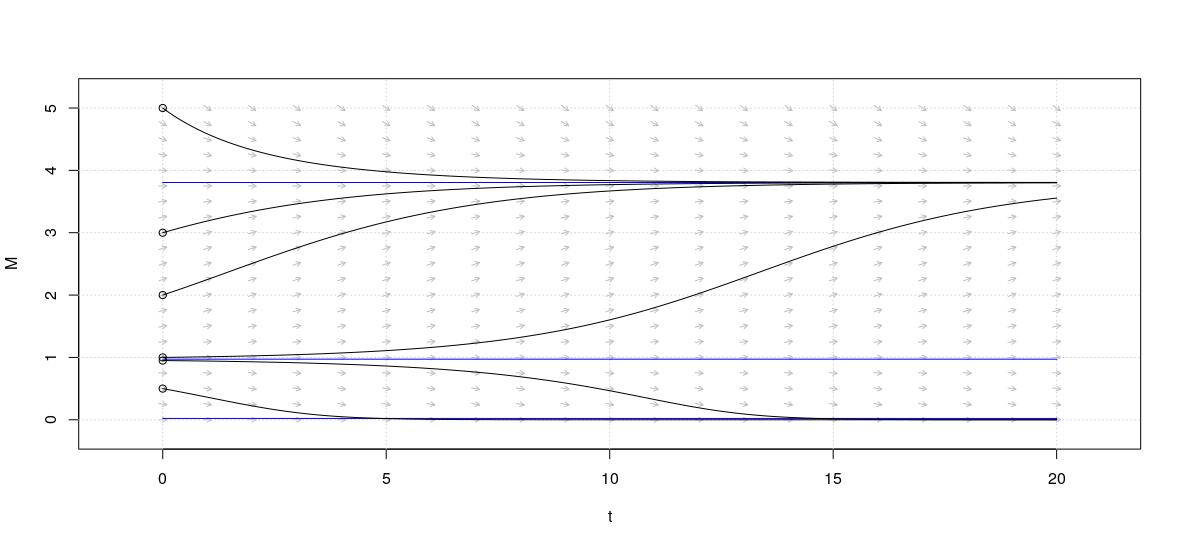
\includegraphics[width=0.99\linewidth]{planophase}
		\caption{}
		\label{f:phase}
	\end{figure}
	








%	{\color{green}
%	Existen dos equilibrios presentes en la solución de la ecuación (\ref{eqequilibrio}). El primero se denomina típicamente \textbf{estable} ya que es la solución endémica.% a la epidemia por geohelmintos, 
%	Este equilibrio es un atractor para un rango de valores de $R_0> R_0 ^*$ (donde $R_0^*$  se refiere al valor de $R_0$ en donde se topan ambos equilibrios). El segundo se conoce típicamente como \textbf{inestable} ya que corresponde a un repulsor en el plano de fase, es decir, una barrera donde los valores de $M$ por encima de ella son atraídos al equilibrio estable y los valores de $M$ por debajo son atraídos hacia el equilibrio de extinción de la enfermedad $M^*= 0$, la cual es la solución trivial de la ecuación (\ref{eqMR0}).
%	}
%	\begin{rem}
%	Una observación importe en este análisis es que el calculo del $R_0$ aquí presentado no es el que se obtiene a partir del calculo del método de la próxima generación.    
%	\end{rem} 
		
\subsection{Saddle-node bifurcation}\label{bifurcacion}
We will show that the basic model developed in the section \ref{ss:structure} presents a saddle node bifurcation. To do this, let us consider the equation (\ref{eqMR0})
%Vamos a demostrar que el modelo clásico desarrollado en la sección \ref{sec:modelclasico} presenta una bifurcación nodo silla. Para ello consideremos la ecuación (\ref{eqMR0})
\begin{equation*}
\dfrac{dm}{dt}=(\mu_h + \mu_p)\left[ R_0  \psi(m)\phi(m) -1 \right] m%\notag es para no tener numero en ecuacion
\end{equation*}
which we compactly denote by
$\dfrac{dm}{dt}=f(m,R_0)$.
A necessary condition for the existence of a saddle node bifurcation in
$(m^{\star},R_0^{\star})$ is
%que vamos a denotar de manera compacta por $	\dfrac{dm}{dt}=f(m,R_0)$. 
%Por la condición necesaria para la existencia de una bifurcación nodo silla en $(m^{\star},R_0^{\star})$
\begin{equation}
\begin{split}
f(m^{\star},R_0^{\star})&=0\qquad\\
\dfrac{\partial f}{\partial m}(m^{\star},R_0^{\star})&=0
\end{split}
\end{equation}
where the first of these conditions is the equilibrium condition \eqref{eqequilibrio} of the system
%donde la primera de estas condiciones es la condición de equilibrio (\ref{eqequilibrio}) del sistema 
\begin{equation*}
\psi(m^{\star};k,z)\phi(m^{\star};k,z)=1/R_0^{\star},
\end{equation*}
and so we get the following equilibrium condition for $m^{\star}$
%y así obtenemos la siguiente condición para el equilibrio $m^{\star}$
\begin{equation}
\frac{\partial }{\partial m}\psi(m^{\star};k,z)\phi(m^{\star};k,z)=0	
\end{equation}
The value of $m$ corresponding to this last condition is
%El valor de $m$ correspondiente con esta ultima condición es 
\begin{equation}
m^{\star}=\dfrac{k\left( \frac{1-z/2}{1-z}\right)^{\frac{1}{k+2}} - k}{-(1-z)\left( \frac{1-z/2}{1-z}\right)^{\frac{1}{k+2}} + (1-z/2)}	
\end{equation}
and its corresponding basic reproductive number is
%y el número reproductivo básico correspondiente es  
\begin{equation}
R_0^{\star}=\left[ \psi(m^{\star};z,k)\phi(m^{\star};z,k)\right]^{-1}
\end{equation}	
%	Recordemos que para la condición de equilibrio (\ref{eqequilibrio}) se verifica que 
%	\begin{equation*}
%	\psi(M^*;z,k)\phi(M^*;z,k)=1/R_0
%	\end{equation*}
%	donde de esta ultima obtenemos que 
%	\begin{equation}
%	\frac{\partial }{\partial M}\psi(M;z,k)\phi(M;z,k)=0	
%	\end{equation}
%	para la condición de equilibrio. 
%	Por lo tanto si denotamos por $R_0^*$ al valor correspondiente a la condición de equilibrio de la ecuación  (\ref{eqequilibrio}) se verifica que 
%	\begin{equation}
%	\dfrac{\partial }{\partial M}f(M^*,R_0^*)=0
%	\end{equation}
%	mostrando así la condición necesaria para la existencia de una bifurcación nodo silla en $(M^*,R_0^*)$.
%Para una condición suficiente para la existencia de una bifurcación nodo silla en $(m^{\star},R_0^{\star})$ y  se puede mostrar que 
A sufficient condition for the existence of a saddle node bifurcation at $(m^{\star},R_0^{\star})$ is
\begin{equation}
\begin{split}
\dfrac{\partial f }{\partial R_0}(m^{\star},R_0^{\star})\neq0\\
\dfrac{\partial^2 f }{\partial m^2}(m^{\star},R_0^{\star})\neq0
\end{split}
\end{equation}
%Si denotamos por $F(M;z,k)=\psi(M;z,k)\phi(M;z,k)$ y 
%Realizando un desarrollo en serie de Taylor de la función $f$ en un entorno de $(m^{\star},R_0^{\star})$ el la ecuación (\ref{eqMR0}) nos queda
By a Taylor series expansion of the function $f$ in a neighborhood of $(m^{\star},R_0^{\star})$, the equation (\ref{eqMR0}) is left
\begin{equation}
{\scriptstyle	\frac{dm}{dt}=f(m^{\star},R_0^{\star})+(m-m^{\star})\frac{\partial f }{\partial m}\big\vert_{(m^{\star},R_0^{\star})}%\delta M
	+(R_0-R_0^{\star}){\frac{\partial f }{\partial R_0}\big\vert_{(m^{\star},R_0^{\star})}}%\delta R_0
	+{\frac {1}{2}}(m-m^{\star})^2{\frac{\partial^2 f }{\partial m^2}}\big\vert_{(m^{\star},R_0^{\star})}%\delta M^{2}
	+\cdots }
\end{equation}
%Por lo tanto localmente en el punto $(m^{\star},R_0^{\star})$ la ecuación es de la forma
Therefore locally at the point $(m^{\star},R_0^{\star})$ the equation is of the form
\begin{equation}
\dfrac{dm}{dt}=\alpha (R_0-R_0^{\star})+\beta (m-m^*)^2
\end{equation}
%donde los valores $\alpha=(\mu_h + \mu_p)\frac{m^{\star}}{R_0^{\star}}$ y $\beta=(\mu_h + \mu_p) R_0 m^{\star} \frac{\partial^2 F}{\partial m^2}(m^{\star})$ con $F(m)= \psi(m;z,k)\phi(m;z,k)$
%obteniendo así la forma normal de una bifurcacion nodo silla.
where the values $\alpha=(\mu_h +\mu_p)\frac{m^{\star}}{R_0^{\star}}$ and $\beta=(\mu_h + \mu_p) R_0 m^{\star} \frac{\partial^2 F}{\partial m^2}(m^{\star})$ with $F(m)= \psi(m;z,k)\phi(m;z, k)$
which is the normal form of a saddle node bifurcation.



\section{A heterogeneous model}
In this section we will consider the most general and realistic case for a host population $H$. Unlike the homogeneous model presented in the previous section, here we present a model that accounts for host population heterogeneity, where subpopulations $H_i$ (e.g., age groups, risk groups, \cite{anderson1992infectious,anderson2014coverage,truscott2014modeling}) have different infection risks. The dynamics of infection for the case of a heterogeneous population is described as follows
\begin{equation}\label{model2}
	\begin{split}
		\dfrac{dm_i}{dt}&=\beta_i \ell - (\mu_h+\mu_p) m_i\\
		\dfrac{d\ell}{dt}&= \frac{\lambda_0}{2}    \sum_i \rho_i \pi_i m_i F(m_i)   - (\mu_{\ell}+\sum_i \beta_i \pi_i ) \ell 
	\end{split}
\end{equation} 
where $\pi_{i}$ is the portion of $H$ to $H_i$ such that $\sum_i \pi_{i}=1$.


\subsection{Equilibria and basic reproduction number} 
From the system \eqref{model2} we obtain that in equilibrium
%Del sistema \eqref{model2} obtenemos que en el equilibrio
%Suponiendo una situación de equilibrio para el reservorio $L$, obtenemos que 
\begin{equation}
	\ell^*=\frac{  \lambda_0}{2 (\mu_{\ell}+\sum_i \pi_i \beta_i  )}   \sum_i \rho_{i} \pi_{i} m_{i} F(m_{i}) 
\end{equation} 
and substituting this in the rest of the equations of the initial system we obtain the following equation for the dynamics of the mean burden $m_{i}$ of the subpopulation $H_{i}$ of hosts
%y reemplazado esto en el resto de las ecuaciones del sistema inicial obtenemos las siguiente ecuación para la dinámica de la carga media $M_{ij}$ de la subpoblación $H_{ij}$ de hospedadores
\begin{equation}
	\begin{split}
		\dfrac{dm_{i}}{dt}=\beta_{i} \frac{\lambda_0}{2 (\mu_{\ell}+\sum_j \pi_j \beta_j  ) }  
		\sum_j   \rho_{j} \pi_{j} m_{j} F(m_{j})  - (\mu_h+\mu_p) m_{i}%\notag es para no tener numero en ecuacion
	\end{split}
\end{equation}
%La carga media del grupo $H_i=\sum_j H_{ij}$ de hospedadores %(con/sin servicios de $H_i$) 
%que denotaremos por $M_i$ viene dada por 
%\begin{equation}
%	M_i=\sum_j p_{ij} M_{ij} 
%\end{equation}
%%donde $p_{ij}$ es la proporción de $H_{ij}$ respecto de $H_i$ tal que $\sum_j p_{ij}=1$, 
%y su dinámica está descripta por 
%\begin{equation}
%	\begin{split}
%		\dfrac{dM_i}{dt}=\left( \sum_j p_{ij}\beta_{ij}\right)  \frac{ \sigma \alpha \lambda}{\mu_L}  \sum_i \pi_i  \sum_j \rho_{ij} p_{ij} M_{ij} F(M_{ij})  - (\mu_H+\mu_W) M_i%\notag es para no tener numero en ecuacion
%	\end{split}
%\end{equation}
%La carga media $m$ de la población total de hospedadores $H=\sum_i H_i$ esta dada por
The mean burden $m$ of the total host population $H=\bigcup_i H_i$ is given by
\begin{equation}
	m=\sum_i \pi_i m_{i} 
\end{equation}
where $\pi_i$ is the portion of the population $H$ corresponding to the subpopulation $H_i$, and which is described by
%donde $\pi_i$ es la porción de la población $H$ correspondiente a la subpoblación $H_i$, y la cual está descripta por 
\begin{equation}
	\begin{split}
		\dfrac{dm}{dt}= \left( \sum_i \pi_i \beta_{i} \right)  
		\frac{ \lambda_0}{2 (\mu_{\ell}+\sum_j \pi_j \beta_j  )}  
		\sum_j \rho_{j} \pi_{j} m_{j} F(m_{j})   -(\mu_{h}+\mu_p) m%\notag es para no tener numero en ecuacion
	\end{split}
\end{equation}
%Suponiendo el diferencial en cero
%de esta ecuación, la carga media de parásitos en equilibrio, $m^*$, para la población total viene dada por
From this equation, the equilibrium mean parasite burden, $m^*$, for the total population is given by
\begin{equation}
	\sum_i \pi_i \frac{ \lambda_0 \rho_{i}}{2 (\mu_{\ell}+\sum_j \pi_j \beta_j  )(\mu_{h}+\mu_p)} 
	\left( \sum_j \pi_{j} \beta_{j} \right) F( m^*_{i}) m^*_{i} - m^*=0 
\end{equation}
%Esta no es una expresión explícita de los equilibrios $m_{i}^*$. Por lo tanto, el valor de los equilibrios solo se pueden resolver numéricamente. 
%Una condición de equilibrio para las cargas medias de cada subpoblación $H_{i}$ viene dada por 
This is not an explicit expression of the equilibria $m_{i}^*$. Therefore, the equilibrium value can only be solved numerically.
An equilibrium condition for the mean burdens of each subpopulation $H_{i}$ is given by
\begin{equation}%\label{eqequilibrio}
	F(m^*_{i})=1/R_0^{i}
\end{equation}
%	\begin{equation}
%	R_{0\rho}=\frac{\sigma \alpha \lambda }{ \mu_L (\mu_H+\mu_M)} (\beta \pi + \hat\beta \hat\pi)\rho
%	\end{equation}
%	donde $R_{0\hat\rho}$ y $R_{0\rho}$ es la contribución del grupo provisto y no provisto de agua y saneamiento respectivamente, para más detalles ver Apéndice (poner referencia).
%	
%	donde $\beta_1=\beta$, $\beta_2=\beta(1-\epsilon_A)$, $\rho_1=\rho$ y $\rho_2=\rho(1-\epsilon_S)$.
%donde definimos por 
%$R_0^{i}=\frac{ \lambda_0 \rho_{i}}{2 (\mu_{\ell}+\sum_j \pi_j \beta_j  )(\mu_{h}+\mu_p)} \left( \sum_j \pi_j\beta_{j} \right) $ 
%al número reproductivo básico propio de cada subpoblación $H_{i}$ que es el número de hembras adultas que surgen 
%%en la población total del hospedador 
%de una hembra adulta de un hospedador de la subpoblación $H_{i}$ en ausencia de los efectos de la denso-dependencia y la probabilidad de apareamiento. 
%Para esta situación de equilibrio obtenemos que la carga media de parásitos de cada subpoblación $H_{i}$ viene dada por $m_{i}^*=\frac{\beta_{i}}{ \sum_j \pi_j\beta_{j} }m^*$.
%El número reproductivo básico general $R_0$ para la población total esta dado por %\cite{diekmann2012mathematical}
where we define by
$R_0^{i}=\frac{ \lambda_0 \rho_{i}}{2 (\mu_{\ell}+\sum_j \pi_j \beta_j )(\mu_{h}+\mu_p)} \left( \sum_j \pi_j\beta_{j} \right) $
to the basic reproductive number of each subpopulation $H_{i}$ which is the number of adult females 
that are born of a 
adult female from a host in subpopulation $H_{i}$ in the absence the effects of density-dependence and the mating probability.
For this equilibrium situation, we obtain that the mean parasite burden of each subpopulation $H_{i}$ is given by $m_{i}^*=\frac{\beta_{i}}{ \sum_j \pi_j\beta_{j } }m^*$.
The general basic reproductive number $R_0$ for the total population is given by %\cite{diekmann2012mathematical}
\begin{equation}\label{valorR0}
	R_{0}=\frac{\lambda_0}
	{2 (\mu_{\ell}+\sum_j \pi_j \beta_j  )(\mu_{h}+\mu_p)}
	\sum_i \pi_i \rho_{i} \beta_{i}   
\end{equation}
%donde suponemos la ausencia de los efectos de la denso-dependencia y la probabilidad de apareamiento \citep{anderson1992infectious}, es decir suponemos en el sistema (\ref{eqmodel2})  la función $F$ igual a la unidad.
where we assume the absence the effects of density-dependence and the mating probability \cite{anderson1992infectious}, that is, we assume in the system \eqref{model2} the function $F$ equal to unity.



%\section{Some numerical results}
%We present some simulations of the system formed by the equations (\ref{model1eq1}) and (\ref{model1eq2}).
%The values of the parameters used in these simulations correspond to the scenario of infection by  \textit{Ascaris lumbricoides} (ascariasis). These parameters are detailed in the Table \ref{table:parametros}, they were extracted from different sources that are mentioned in this table.
%
%%En esta sección presentamos algunas simulaciones del sistema formado por las ecuaciones (\ref{model1eq1}) y (\ref{model1eq2}). 
%%Los valores de los parámetros utilizados en estas simulaciones corresponden al escenario de la infección por Ascaris \textit{lumbricoides} (ascariasis) en una población con parámetro de dispersión $k$ correspondiente a la distribución de parásitos. Estos parámetros se encuentra detallados en la Tabla \ref{table:parametros}, los mismos fueron extraídos de diferentes fuentes que se mencionan en esta tabla.
%\begin{table}[h!]
%	\centering	
%	\begin{tabular}{llc} 	
%		Parameter & Value & Source \\
%		\hline 
%		dispersion parameter, $k$ & $0.7$ & \cite{elkins1986epidemiology}\cite{hall1999distribution}\\ 
%		%\hline 
%		density dependence , $\gamma$ & $0.08$ & \cite{holland1989epidemiology}\\ 
%		%denso dependencia , $\lambda_0$ & 0.93 & \\
%		average parasite lifespan, $1/\mu_M$ & $1$ año & \cite{croll1982population}\\
%		average egg survival time, $1/\mu_L$ & $2$ meses & \cite{larsen1999seasonal}\\
%		average host lifespan, $1/\mu_H$ & $70$ años & - \\
%		relative contact rate, $\beta$ & $1$ & - \\
%		relative contribution rate, $\rho$ & $1$ & -
%		%proporción sexual, $\varrho$ & 0.574 & \cite{seo1979egg}
%		%tasa relativa de contacto  de niños, $\beta_n$ & 2/3&\\
%		%tasa relativa de contribución de niños, $\rho_n$ & 2/3&\\
%		%fracción de población de niños, $n_n$ & 0.3	&
%	\end{tabular}
%	\caption{Tabla de parámetros}
%	\label{table:parametros}
%\end{table}
%\begin{figure}[h!]
%	\centering
%	%\includegraphics[width=0.99\linewidth]{model1v2}
%	\caption{Serie de tiempo de la carga media de parásitos y el reservorio para diferentes valores de $R_0$. } 
%	\label{fig:model1}
%\end{figure} 
%%{\color{red}COMENTAR EL NODO SILLA DE LA SIMULACION}
%La Figura \ref{fig:model1} muestra el comportamiento de la carga media de parásitos $M$ y el reservorio $L$ para diferentes valores del número reproductivo básico $R_0$. La bifurcación nodo ensilladura del sistema correspondiente a esta simulación se produce en el punto $(M^*,R_0^*)\simeq(1.94,1.97)$. Los valores de equilibrio de la carga media de parásitos para los diferentes valores de $R_0$  se obtienen a partir de la ecuación (\ref{eqequilibrio}). Para los valores de $R_0$ mayores que uno se observa que la infección por geohelmintos es endémica. Para el valor de $R_0=1$ se produce la extinción de la infección $M\to 0$.


\section*{Aknowledgements}
This work was partially supported by grant CIUNSA 2018-2467. JPA is a member of the CONICET. GML is a doctoral fellow of CONICET.

\section*{Conflict of Interest}
The authors have declared no conflict of interest.

%Reference
\bibliographystyle{apa}
\bibliography{biblio}	

\end{document}
